En esta primera práctica nos familiarizaremos con las interfaces gráficas del
qgis y de R-studio. Para esto comenzaremos a analizar la imagen correspondiente
a la zona de estudio del año 2015 desde el punto de vista espectral. Son
nuestros objetivos

\begin{itemize}
    \item Poder cargar una imagen en qgis.
    \item Digitalizar coberturas en qgis.
    \item Poder cargar un archivo raster y uno vectorial en R.
    \item Realizar un análisis estadistico de la imagen como un todo y de las
        distintan coberturas digitalizar en R.
\end{itemize}
\subsection{Exploración de imagenes con el qgis}

Comenzamos abriendo la imagen \file{LC82240782016304LGN00.vrt} que se encuentra
en la carpeta \file{raster\_data,LC82240782016304}. Esta image  corresponde al 
departamento de Iguazu en la provincia de corriente. La misma fue obtenida por 
el satelite Landsat 8 durante el mes de noviembre de 2016.
 
Para esto vamos al menú \menu{Capa, Añadir capa, Añadir capa ráster}. Navegamos 
hasta la carpeta \file{raster\_data/LC8224078201630} y abrimos el archivo
\file{LC82240782016304LGN00.vrt}. Una vez abierto el mismo podremos encontrarlo
en el \menu{Panel de capas} de q-gis donde podremos manejar la visualización del
mismo y estudiar las propiedades de dicha capa.

\begin{figure}[htb]
\begin{center}
    
\includegraphics[scale=0.5]{move.png}
\end{center}
\caption{Herramientas para moverse dentro de la imagen. De izquierda a derecha:
    1. Desplazar mapa, 2. Desplazar mapa a la seleccion, 3. Acercar zum, 4.
    Alejar zum, 5. Zum a la resolucion nativa, 6. Zum general, 7. Zum a la
    seleccion, 8. Zum a la capa, 9. Zum anterior, 10. Zum siguiente, 11.
    Actualizar.}
\label{fig:move}
\end{figure}

Para realizar cambiar la visualizacion y explorar los datos de una capa, hacemos
click derecho sobre la misma y luego seleccionamos la opciopn
\menu{Propiedades}. Dentro de las propiedades de la capa podemos ir a la pestaña
\menu{General} para ver datos como el nombre de la capta\footnote{Es un buen
momento para ponerle uno mas sencillo}, la cantidad de filas y columnas del
archivo, el valro digital no valido, el sistema de referencias de coordenadas
entro otros. 

\begin{figure}[htb]
\begin{center}
    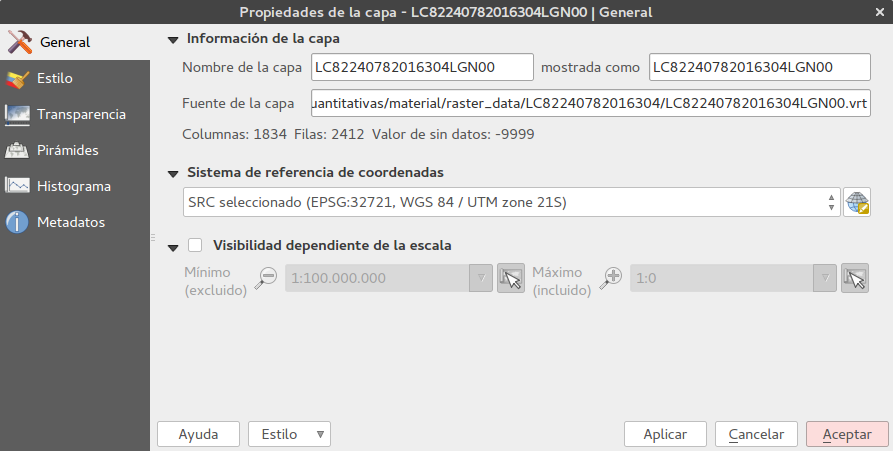
\includegraphics[scale=0.3]{general.png}
\end{center}
\caption{Pestaña general de propiedades de una capa. En la misma se pueden ver
    los datos mas importantes sobre la misma como la cantidad de filas y
    columnass, el nombre y el sistema de referencia de coordenadas.}
\label{fig:general}
\end{figure}

Podemos ir luego a la pestaña de estilo para cambiar la visualizacion de la
imagen. En la misma podemos elegir de que color mostraremos cada una de las
capas ademas de elegir el tipo de realce que deseamos aplicar. Es importante
remarcar en este caso que una vez elegidas las badnas debemos hacer click en el
boton \menu{Cargar} para seleccionar los valores maximos y minimos de las
bandas para el realcec.

\begin{figure}[htb]
\begin{center}
    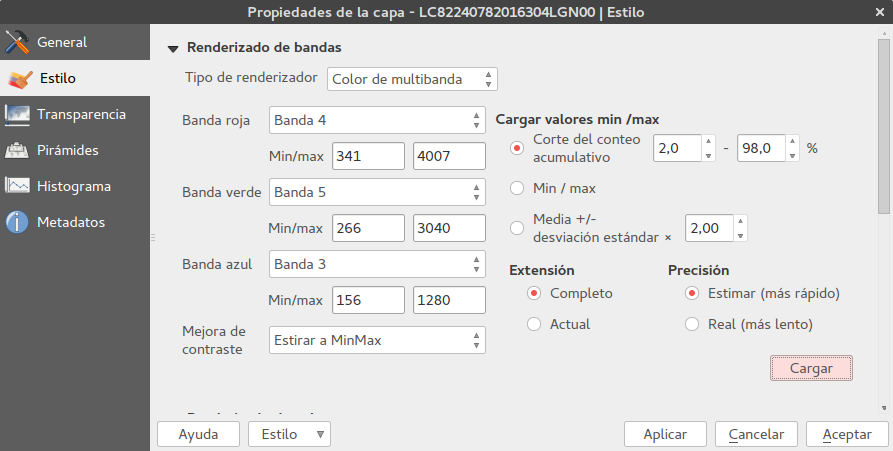
\includegraphics[scale=0.3]{estilo.png}
\end{center}
\caption{Estilos de visualizacion de una capa raster. Los estilos posibles son:
    1. Color de multibanda, 2. En paleta, 3. Unibanda gris, 4. Unibanda
    pseudocolor. Puede explorar cada uno por separado ya que todos tendran
    distintas utilidades.}
\label{fig:estilo}
\end{figure}

\begin{act} 
    Cambie la combinación de bandas de la imagen L8 y muévase  dentro de la
    misma. Identifique zonas de coberturas uniformes. Pruebe cambiar de
    combinacion de bandas y decida si dichas zonas siguen siendo uniformes luego
    del cambio.
\end{act}

\begin{act}
    Encuentre el sistema de coordenadas en el cual se encuentra la imagen.
\end{act}

Para identificar la informacion correspondiente a un punto en el espacio podemos
utilizar la herramienta \menu{Identificar un objeto espacial}. Al habilitarla y
hacer click sobre un punto de la imagen veremos datos de la misma como por
ejemplo los valores de reflectancia del pixel seleccionado. Dichos valores
pueden mostrarse como Arbol, Tabla o Grafo segun como sea mass comodo.

\begin{figure}[htb]
\begin{center}
    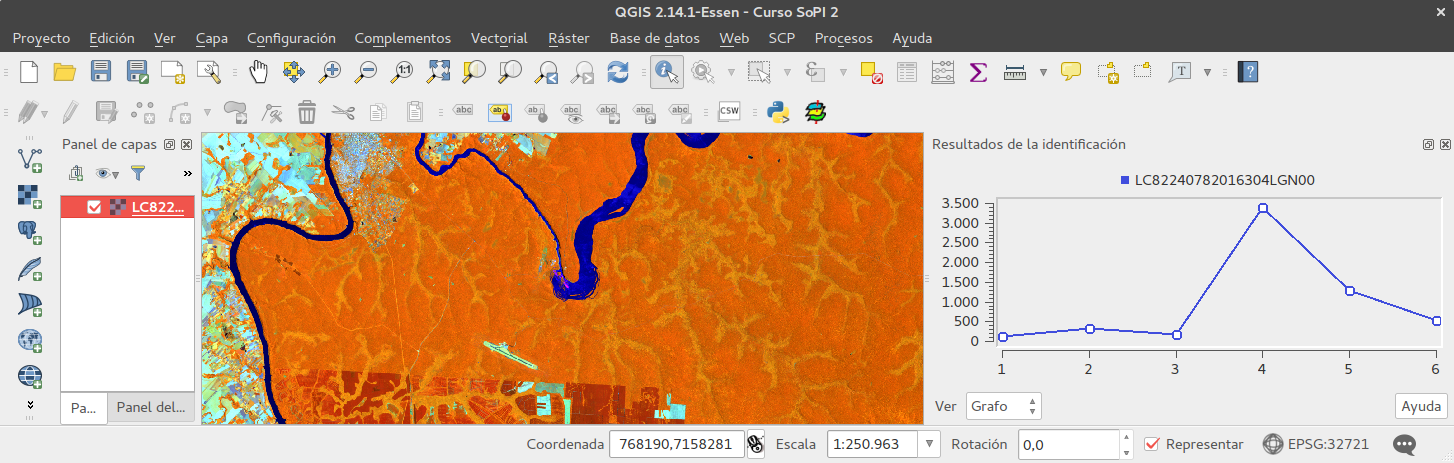
\includegraphics[scale=0.3]{grafo.png}
\end{center}
\caption{Identificacion de un pixel correspondiente a la selva paranaense
    mostrada como grafo. }
\label{fig:grafo}
\end{figure}

\begin{act}
   Utilizando la herramienta identificar objetos espaciales encuentre los
   valores de reflectancia de distintas coberturas. Grafique estos  valores en
   una firma espectral y en el espacio de fases nirrojo.
\end{act}

\subsection{Creacion de capas vectoriales}

Veamos ahora como crear capas vectoriales con las cuales podamos extraer
informacion sobre nuestra zona.

Con la herramienta nueva capa de archivo shape es posible digitalizar zonas de
la imagen para su posterior analisis. Para esto puede hacer click en el boton
del panel lateral. Podemos agregar los campos que sean necesarios para nuestra
capa vectorial en este momento. Crearemos al menos los campos MC\_ID como entero
de longitud 1 y Comment como texto de 80 caracteres. Guardela en la carpeta 
\file{vector\_data/} con el nombre \file{firmas.shp}. Recuerde elegir el sistema 
de coordenadas correspondiente a la imagen anterior. 

\begin{figure}
\begin{center}
    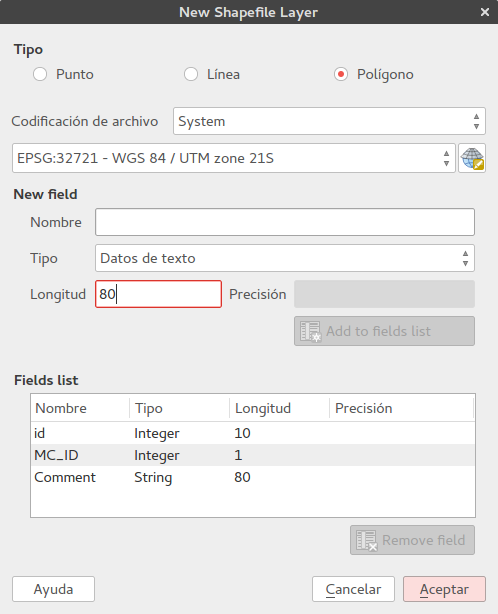
\includegraphics[scale=0.3]{new_shape.png}
\end{center}
\caption{Creacion de una nueva capa vectorial. Se agregan campos que seran de
    interes para comparar las firmas espectrales. }
\label{fig:newshape}
\end{figure}


Una vez creada la nueva capa podemos utilizar la barra de herramientas de qgis
para agregar nuevas geometrias a la misma. Para esto hacemos click en el boton
de agregar geometrica y digitalizamos una zona uniforme dentro de la imagen. 
\begin{figure}
\begin{center}
    
\includegraphics[scale=0.5]{shapetool.png}
\end{center}
\caption{Herramientas de edición vectorial. De izquierda a derecha: 1. Conmutar
    edicion, 2. Guardar cambios a la capa, 3. Añadir objeto espacial, 4. Añadir
    cadena circular, 5. Mover objeto espacial, 6. Herramienta de nodos, 7.
    Borrar lo seleccionado, 8. Cortar objetos espaciales, 9. Copiar objetos
    espaciales, 10. Pegar objetos espaciales.}
\label{fig:shapetool}
\end{figure}

Al terminar de acerlo qgis pedira un numero de ID para la capa que debe ser
correlativo. Además podremos ingresar en este momento los valores del resto de
los campos de nuestro objeto espacial.

\begin{figure}
\begin{center}
    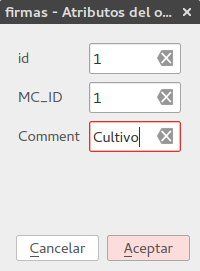
\includegraphics[scale=0.3]{new_poli.png}
\end{center}
    \caption{Valores de los campos del nuevo poligono creado.}
    \label{fig:newpoli}
\end{figure}

\begin{act}
   Digitalize coberturas uniformes dentro de la imagen. Recuerde obtener al
   menos una por cada categoria de uso y cobertura presente dentro de la misma.
\end{act}

En caso de desear cambiar la visualizacion de la capa vectorial, podemos entrar
a las propiedades de la misma\footnote{Pueded utilizar el estilo precargado
ubicado en la carpeta \file{aux\_data}}. Ademas podemos acceder a la tabla de
datos de la capa vectorial haciendo click derecho sobre la misma y eligiendo la
opcion \menu{Abrir tabla de atributos}.

\subsection{Exploracion raster en R}
Busquemos ahora como abrir y trabajar con las imagenes satelitales en R. Para
esto comenzamos cargando las librerias que vamos a utilizar con el comando
\texttt{library(raster)}. 

Además, deberemos situar nuestra carpeta de trabajo donde se encuentran las
carpetas que descargamos. Para esto nos movemos en el explorar de archivos
hasta la misma y hacemos click en usar la carpeta como carpeta de trabajo.

\begin{figure}
\begin{center}
    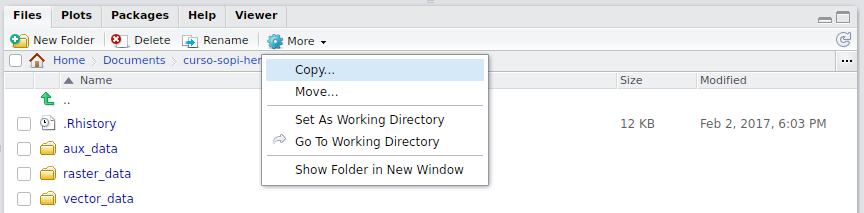
\includegraphics[scale=0.3]{setwd.png}
\end{center}
\caption{Configuracion del directorio de trabajo desde la interfaz grafica.}
\label{fig:setwd}
\end{figure}

Tambien podemos utilizar el comando \texttt{setwd()} para configurar el
directorio de trabajo.

Una vez en dicha carpeta, existen varias maneras de abrir una imagen segun
queramos hacerlo solo para una banda, varias bandas en archivos separados o un
solo archivo multibanda.

Los comandos para esto son \texttt{raster}, para abrir una unica banda,
\texttt{brick}, para abrir un archivo multibanda, y \texttt{stack} para abrir
distinas bandas por separado. Veamos algunos ejemplo de esto:

\begin{exa}
    Abrimos la imagen completa del archivo de Landsat 8 y consultamos sus 
    propiedades. 
    \begin{lstlisting}
    ref.2016 <- brick("raster_data/LC82240782016304/LC82240782016304LGN00.vrt")
    ref.2016
    \end{lstlisting}
    obtenemos de resultado el siguiente text
    \begin{Verbatim}[fontsize=\small]
    class       : RasterBrick 
    dimensions  : 2412, 1834, 4423608, 6  (nrow, ncol, ncell, nlayers)
    resolution  : 30.00402, 30.00265  (x, y)
    extent      : 731118.6, 786146, 7101531, 7173897  (xmin, xmax, ymin, ymax)
    coord. ref. : +proj=utm +zone=21 +south +datum=WGS84 +units=m +no_defs 
                  +ellps=WGS84 +towgs84=0,0,0 
    data source : ./material/raster_data/LC82240782016304/LC82240782016304LGN00.vrt 
    names       : LC82240782016304LGN00.1, LC82240782016304LGN00.2, ... 
    min values  :                     -33,                     192, ... 
    max values  :                    2774,                    3265, ... 
    \end{Verbatim}
    En el podemos ver la clase a la que corresponde el archivo abierto, en este
    caso un \emph{RasterBrick}, las dimensiones, el tamaño de pixel, extension
    de la capa, proyeccion, cual es la ruta al archivo que abrimos, las bandas y
    sus valores maximos y minimos.
\end{exa}

Una vez abierta la imagen en el R podemos empezar a trabajar con la misma
utilizando distintos comandos. 

\begin{exa}
    Veamos primero como cambiar los nombres de las bandas por defecto, cambiar la
    imagen a numeros en reflectancia entre 0 y 1 y luego guardarla nuevamente. Para
    eso ejecutamos el siguiente codigo.
    \begin{lstlisting}
    ref.2016 <- brick(filename)
    names(ref.2016) <- c("blue","gree","red","nir","swir1","swir2")
    ref.2016 <- ref.2016/1e4
    rasterOptions(addheader = "ENVI")
    writeRaster(ref.2016,"raster\_data/processed/ref2016")
    \end{lstlisting}

    Analicemos el codigo linea por linea. 
    \begin{itemize}
    \item La primera de ellas abre la imagen como  un raster de multiples bandas. 
    \item La segunda, cambia los nombres de cada banda a los que figuran en la 
          lista entre parentesis. Es importante resaltar que el numero de nombres 
          debe ser el mismo que el de bandas. 
    \item En tercer lugar convertimos el archivo de numeros enteros entre 0 y 
          10000 a numeros entre 0 y 1.
    \item La cuenta linea es necesaria correrla una sola vez por sesion. La misma
          agrega el header de ENVI a nuestro output para poder abrir el archivo
          desde qgis
      \item La sexta linea guarda el archivo raster con el nombre \file{ref2016} 
    \end{itemize}
    podemos ademas graficar tanto una combinacion de bandas en qgis
    \begin{lstlisting}
    plotRGB(ref.2016,r=4,g=5,b=3, stretch='lin')   
    \end{lstlisting}
    Obtenemos como resultado
    \begin{figure}
    \begin{center}
        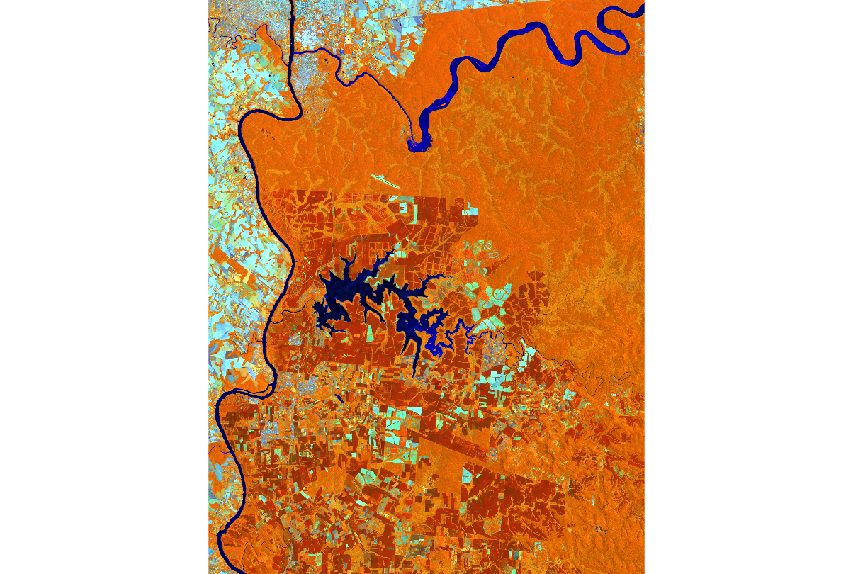
\includegraphics[scale=0.3]{plot453.png}
    \end{center}
    \caption{Combinacion de bandas nir-swir1-red en R.}
    \label{fig:}
    \end{figure}
    como tambien todas las bandas por separado
    \begin{lstlisting}
    plotRGB(ref.2016) 
    \end{lstlisting}
    obtenemos como resultado
    \begin{figure}
    \begin{center}
        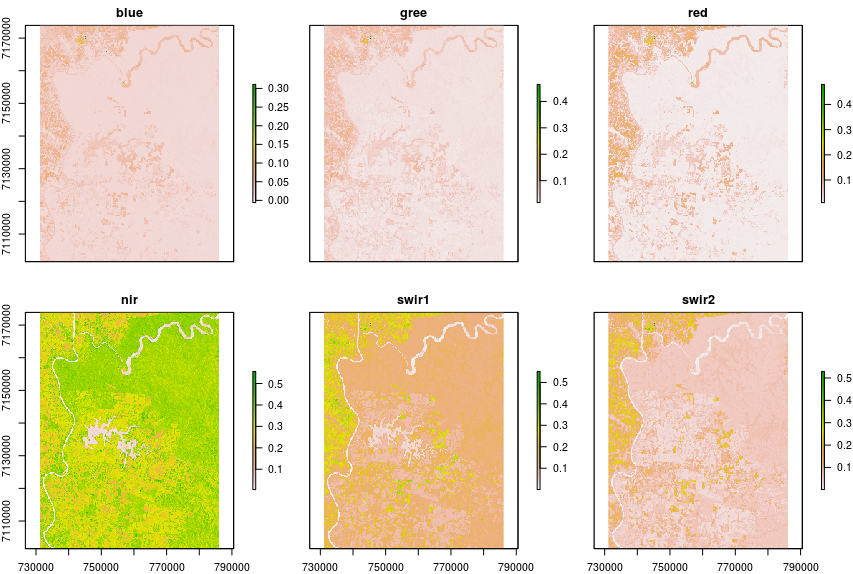
\includegraphics[scale=0.3]{plotband.png}
    \end{center}
    \caption{Grafico de bandas con realce automatico para cada una.}
    \label{fig:plotband}
    \end{figure}
    
\end{exa}
 
\begin{act} 
   Abra el archivo vrt en qgis y vuelva a mirar la firma espectral para 
   distintas coberturas. Entre que valores se encuentra ahora las mismas.
\end{act}

\begin{exa}

    Hagamos un poco de analisis ahora sobre la imagen. En primer lugar podemos
    calcular un sumario de la estadistica de nuestra imagen
    \begin{lstlisting}
    summary(ref.2016)   
    \end{lstlisting}
    obtenemos como resultado
    \begin{Verbatim}[fontsize=\small]
               blue   gree    red     nir   swir1   swir2
    Min.    -0.0278 0.0000 0.0000 -0.0128 -0.0069 -0.0038
    1st Qu.  0.0128 0.0328 0.0184  0.2763  0.1198  0.0493
    Median   0.0138 0.0362 0.0203  0.3287  0.1365  0.0572
    3rd Qu.  0.0170 0.0450 0.0329  0.3557  0.1644  0.0749
    Max.     0.5548 0.8257 0.8034  0.7542  0.9181  0.9446
    NA's     0.0000 0.0000 0.0000  0.0000  0.0000  0.0000
    \end{Verbatim}
    Para comenzar podemos calcular los histogramas de todas las bandas con el 
    comando
    \begin{lstlisting}
    hist(ref.2016) 
    \end{lstlisting}

    y el scatter plot entre dos bandas como

    \begin{lstlisting}
    plot(l8$red, l8$blue)    
    \end{lstlisting}

    en caso de querer todos los scatterplots e histogramas en un solo grafico
    podemos hacerlo con el comando
    \begin{lstlisting}
    pairs(l8)
    \end{lstlisting}
    \end{exa}


\subsection{Manejo vectorial en R}

Hasta ahora estamos analizando la imagen completa. Podemos sin embargo analizar
solo sectores concretos de la imagen muestreandola en funcion de un archivo
vectorial. Tambien sera posible muestrar la imagen pos zonas definidas por otro
raster pero veremos esto mas adelante.

Para poder trabajar con vectores en R utilizaremos la libreria
\texttt{library(rgal)}.

\begin{exa}
    Podemos leer un vector como
    \begin{lstlisting}
    firmas <- readOGR(dsn="vector\_data/", layer="firmas")
    \end{lstlisting}
    Notamos en este caso que debemos indicar por separado la carpeta que
    contiene al shapefilee en \emph{dsn} y el nombre de la capa que queremos
    abrir como \emph{layer}.

    Podemos mostrar las propiedades del vector ejecutando el comando

    \begin{lstlisting}
    vector
    \end{lstlisting}

    obteniendo como resultado
    \begin{Verbatim}[fontsize=\small]
    class       : SpatialPolygonsDataFrame 
    features    : 8 
    extent      : 738692.8, 767774.6, 7133396, 7165265  (xmin, xmax, ymin, ymax)
    coord. ref. : +proj=utm +zone=21 +south +datum=WGS84 +units=m +no_defs
                  +ellps=WGS84 +towgs84=0,0,0 
    variables   : 3
    names       : id, MC_ID,       Comment 
    min values  :  0,     1,          Alto 
    max values  :  9,     8, Suelo desnudo 
    \end{Verbatim}  

    Podemos graficar los vectores obtenidos en R junto aa la imagen de base como

    \begin{lstlisting}
    plotRGB(ref.2016, stretch="lin")
    plot(firmas,add=TRUE,col='red')
    \end{lstlisting}
    donde la primera linea grafica la imagen de fondo y la segunda agrega el
    el shapefile sobre la misma.
\end{exa}

\begin{act} 
    Muestre las propiedades de la capa raster y el vector abiertos y verifique
    que los mismos se encuentren en el mismo sistema de coordenadas.
\end{act}

Por ultimo mostremos como extraer datos de un archivo raster y veamos un par de
ejemplo concretos. La funcion que nos permite extrar datos de un raster segun
un vector es \texttt{extract} que toma dos argumentos, el vector que queremos
utilizar y la capa raster sobre la cual hacer la consulta.

Veamos algunos ejemplos

\begin{exa}
    Graficar en un scatterplot de dos bandas mostrando la zona del espacio 
    ocupada por una cobertura.
    \begin{lstlisting}
    datos <- extract(ref.2016,firmas)
    \end{lstlisting}
    de esta forma realizamos la extraccion de todos los datos de la imagen a una
    lista
    \begin{lstlisting}
    plot(ref.2016$red, ref.2016$nir)
    points(as.data.frame(datos[1])$red, as.data.frame(datos[1])$nir,col="green",
           pch = ".")
    \end{lstlisting}
    obteniendo como resultado
    \begin{figure}
    \begin{center}
        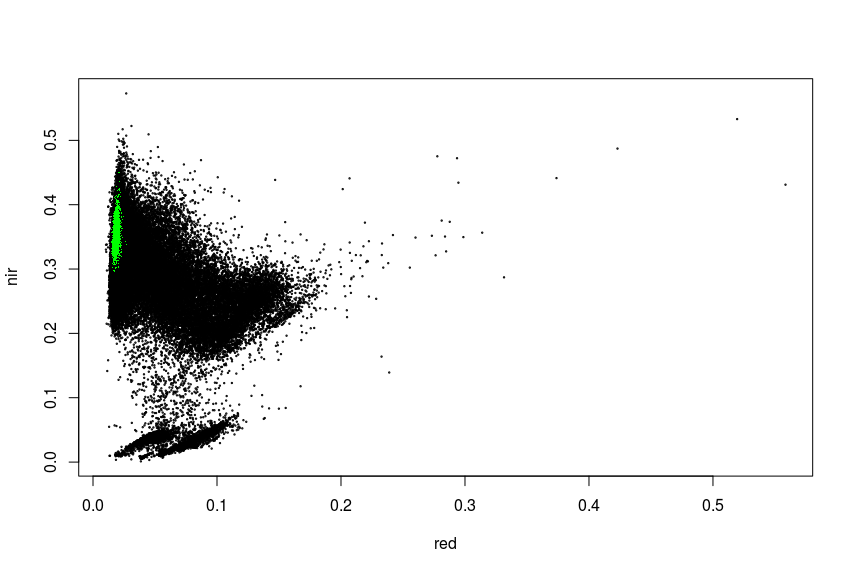
\includegraphics[scale=0.3]{plot-red-nir-zone.png}
    \end{center}
    \caption{Resultado del scatterplot para las bandas roja y nir. Se muestra en
        verde datos correspondientes a la selva paranaense.}
    \label{fig:}
    \end{figure}
    
\end{exa}

La funcion \texttt{extract} nos permite tambien aplicar una funcion a los datos
extraidos antes de entregarlos al usuario. Veamos como usarla para calcular
datos de interes sobre las coberturas.

\begin{exa}
     Extraer los promedios y desvios standar de un raster y agregarlos a un
     vector. Primero extraemos los valores de promedio y desvio
     \begin{lstlisting}
     promedio <- extract(ref.2016,firmas,fun=mean)
     desvio <- extract(ref,firmas,fun=sd)
     \end{lstlisting}
     renombramos luego las columnas como promedio y devio seguido de la banda a
     la que pertenecen,
     \begin{lstlisting}
     colnames(promedio) <- paster("mean",colnames("promedio"),sep="_")
     colnames(desvio) <- paster("sd",colnames("desvio"),sep="_")
     \end{lstlisting}
     finalmente agregamos los archivos a un nuevo shapefile
     \begin{lstlisting}
     firmas@data <- cbind(firmas@data,promedio,desvio)
     writeOGR(firmas, sdn="vector_data/processed/,"firmas_datos",
              driver="ESRI Shapefile")
     \end{lstlisting}
\end{exa}

Por ultimo, veamos como usar una capa vectorial para graficar para extraer las
firmas espectrales y graficarlas para distintas coberturas

\begin{exa}
     Graficar las firmas espectrales en funcion de la longitud de onda para cada
     geometria de un vector. Utilizaremos en este caso una nueva libreria,
     \texttt{reshape2}

     Comenzamos convirtiendo en dataframe a nuestros promedios donde cada
     columna corresponde a una firma espectral
     \begin{lstlisting}
     df <- t(promedio)
     colnames(df) <- vector@data$Comment
     \end{lstlisting}
     Agregamos luego una columna con las longitudes de onda en nanometros. Luego
     reformamos el dataframe para que podamos subsetearlo, poniendo finalmente
     los nombres a cada columna
     \begin{lstlisting}
     df$wl <- as.matrix(c(485,560,660,830,1650,2215))
     df <- melt(df,id.vars="wl", variable.name="cobertura")
     names(df) <- c("wl","Cobertura","Reflectancia")
     \end{lstlisting}
     si mostramos el dataframe, el resutado debería ser similar al siguiente
     \begin{Verbatim}[fontsize=\small]
          wl     Cobertura Reflectancia
     1   485          Alto  0.012926561
     2   560          Alto  0.034730646
     3   660          Alto  0.018491884
     4   830          Alto  0.354564681
     5  1650          Alto  0.133750642
     ...
     \end{Verbatim}
     repetimos el proceso para los desvios standar
     \begin{lstlisting}
     dfd <- t(desvio)
     colnames(dfd) <- vector@data$Comment
     dfd$wl <- as.matrix(c(485,560,660,830,1650,2215))
     dfd <- melt("wl","Cobertura","Desvio")
     df$desvio <- dfd$desvio
     df$MC_ID <- as.character(vector@data$MC_ID[match(df$Cobertura,
                              vector@data$Comment)])
     \end{lstlisting}
     el resultado sera ahora
     \begin{Verbatim}[fontsize=\small]
         wl     Cobertura Reflectancia       Desvio
     1   485          Alto  0.012926561 0.0007772473
     2   560          Alto  0.034730646 0.0018113004
     3   660          Alto  0.018491884 0.0011561294
     4   830          Alto  0.354564681 0.0166801398
     5  1650          Alto  0.133750642 0.0075157929
     ...
     \end{Verbatim}
     Veamos algunas opciones para generar ahora los graficos. En primer lugar
     pondremos todas las firmas juntas, separadas por color
     \begin{lstlisting}
     xyplot(Reflectancia~wl, data=df, groups = Cobertura,
            auto.key=list(space="top", columns=4), 
            ty=c("l", "p"))
     \end{lstlisting}
     Aqui la primer linea dice que grafiquemos la reflectancia como funcion de
     la longitud de onda, obteniendo los datos del dataframe df y agrupandolos
     segun la columna cobertura. La siguiente linea agrega la leyenda en la
     parte superior de la figura y con 4 columnas. Por ultimo en la tercer linea
     pedimos que el grafico tenga lineas y puntos.
     \begin{figure}
     \begin{center}
         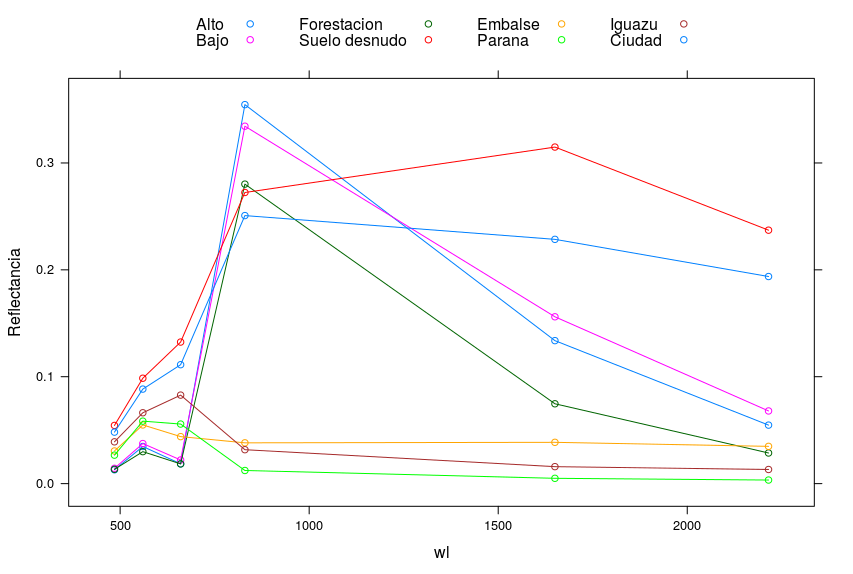
\includegraphics[scale=0.3]{spectra-1.png}
     \end{center}
     \caption{Firmas espectrales}
     \label{fig:spectra-1}
     \end{figure}
     Si queremos agruparlo por categoria de uso y cobertura cambiamos la formula
     \texttt{Reflectancia ~ wl} por \texttt{Reflectancia ~ wl | MC\_ID}
     \begin{lstlisting}
     xyplot(Reflectancia~wl | MC_ID, data=df, groups = Cobertura,
            auto.key=list(space="top", columns=4), 
            ty=c("l", "p"))
     \end{lstlisting}
     y finalmente si queremos graficar solo un subset de los daatos
     \begin{lstlisting}
     xyplot(Reflectancia~wl | MC_ID, data=df, groups = Cobertura,
            auto.key=list(space="top", columns=4), ty=c("l", "p"),
            subset = Cobertura %in% c("Alto","Bajo"))
     \end{lstlisting}
     \begin{figure}
     \begin{center}
         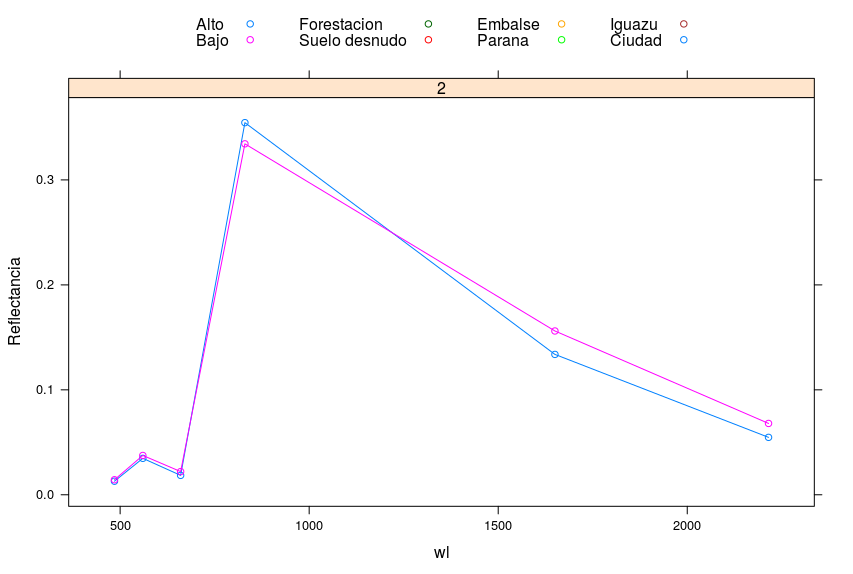
\includegraphics[scale=0.3]{spectra-2.png}
     \end{center}
     \caption{Firmas espectrales}
     \label{fig:spectra-1}
     \end{figure}
 \end{exa}

\begin{act}
    Grafique la media y el desvio standar para las distintas coberturas que pudo
     identificar en el punto uno. 
\end{act}
